\documentclass[11pt]{article}

\usepackage[margin=1in]{geometry}
\usepackage{amsmath,amssymb,amsthm}
\usepackage[T1]{fontenc}
\usepackage{lmodern}
\usepackage{microtype}
\usepackage{graphicx}

\title{\vspace{-1.5em}Why So Much Love for the Conditional Expectation Function?}
\author{Estimation I}
\date{}

\begin{document}
\maketitle
\vspace{-2.5em}

In applied work, the estimand is very often an \emph{average}: average dictator tenure, the average treatment effect, or the average treatment effect on the treated. More generally, much of econometrics is organized around the \emph{conditional expectation function} (CEF). Why this object, rather than the conditional median, mode, or some other summary?

One answer is predictive. The CEF
\[
m(x)=E[Y\mid X=x]
\]
minimizes mean squared prediction error:
\[
m(\cdot)\in \arg\min_{g(\cdot)} E[(Y-g(X))^2].
\]
So if squared loss is the relevant criterion, the CEF is the optimal predictor. But this only shifts the question: why squared loss rather than absolute loss, under which the conditional median would be optimal? Most applied researchers do not have a deep substantive defense of one loss function over another.

A deeper answer is mathematical. The mean is not just one summary among many. It is the one that makes prediction especially tractable, because of the space it lives in.

A \emph{normed space} is a vector space equipped with a function \(\|\cdot\|\) that measures the ``size'' of each element---a norm. When we measure prediction error by squared loss, \(E[(Y - g(X))^2]\), the natural notion of size is \(\|Z\| = (E[Z^2])^{1/2}\), and the resulting space of random variables with finite second moments is called \(L^2\). But \(L^2\) is more than just a normed space. Its norm happens to come from an inner product, \(\langle Y,Z\rangle = E[YZ]\), which makes \(L^2\) a \emph{Hilbert space}. That inner product gives us angles, orthogonality, and projections---and with them, the CEF is the projection of \(Y\) onto the space of functions of \(X\).

That geometric interpretation yields the familiar orthogonality condition
\[
Y=E[Y\mid X]+\varepsilon,
\qquad E[\varepsilon\mid X]=0,
\]
and the variance decomposition
\[
\operatorname{Var}(Y)
=
\operatorname{Var}(E[Y\mid X])
+
E[\operatorname{Var}(Y\mid X)].
\]
These properties are why the CEF provides a unique, stable, and analytically tractable summary of how \(X\) relates to \(Y\).

All of this rests on a single algebraic identity---the parallelogram law---which holds whenever a norm comes from an inner product. Understanding this identity is the key to seeing why the geometry of the CEF works at all, and why it fails for other loss functions.

\subsection*{What is the parallelogram law?}

The parallelogram law is the identity that characterizes norms coming from an inner product. For any two vectors \(u\) and \(v\) in an inner product space,
\[
\|u+v\|^2 + \|u-v\|^2 = 2\bigl(\|u\|^2 + \|v\|^2\bigr).
\]
Geometrically, \(u+v\) and \(u-v\) are the two diagonals of the parallelogram formed by \(u\) and \(v\). The identity says that the sum of the squared diagonal lengths always equals twice the sum of the squared side lengths. Figure~\ref{fig:parallelogram} illustrates this with a concrete example: the diagonal areas (red, \(25+5=30\)) exactly equal twice the side areas (blue, \(2\times 10 + 2\times 5 = 30\)).

\begin{figure}[ht]
\centering
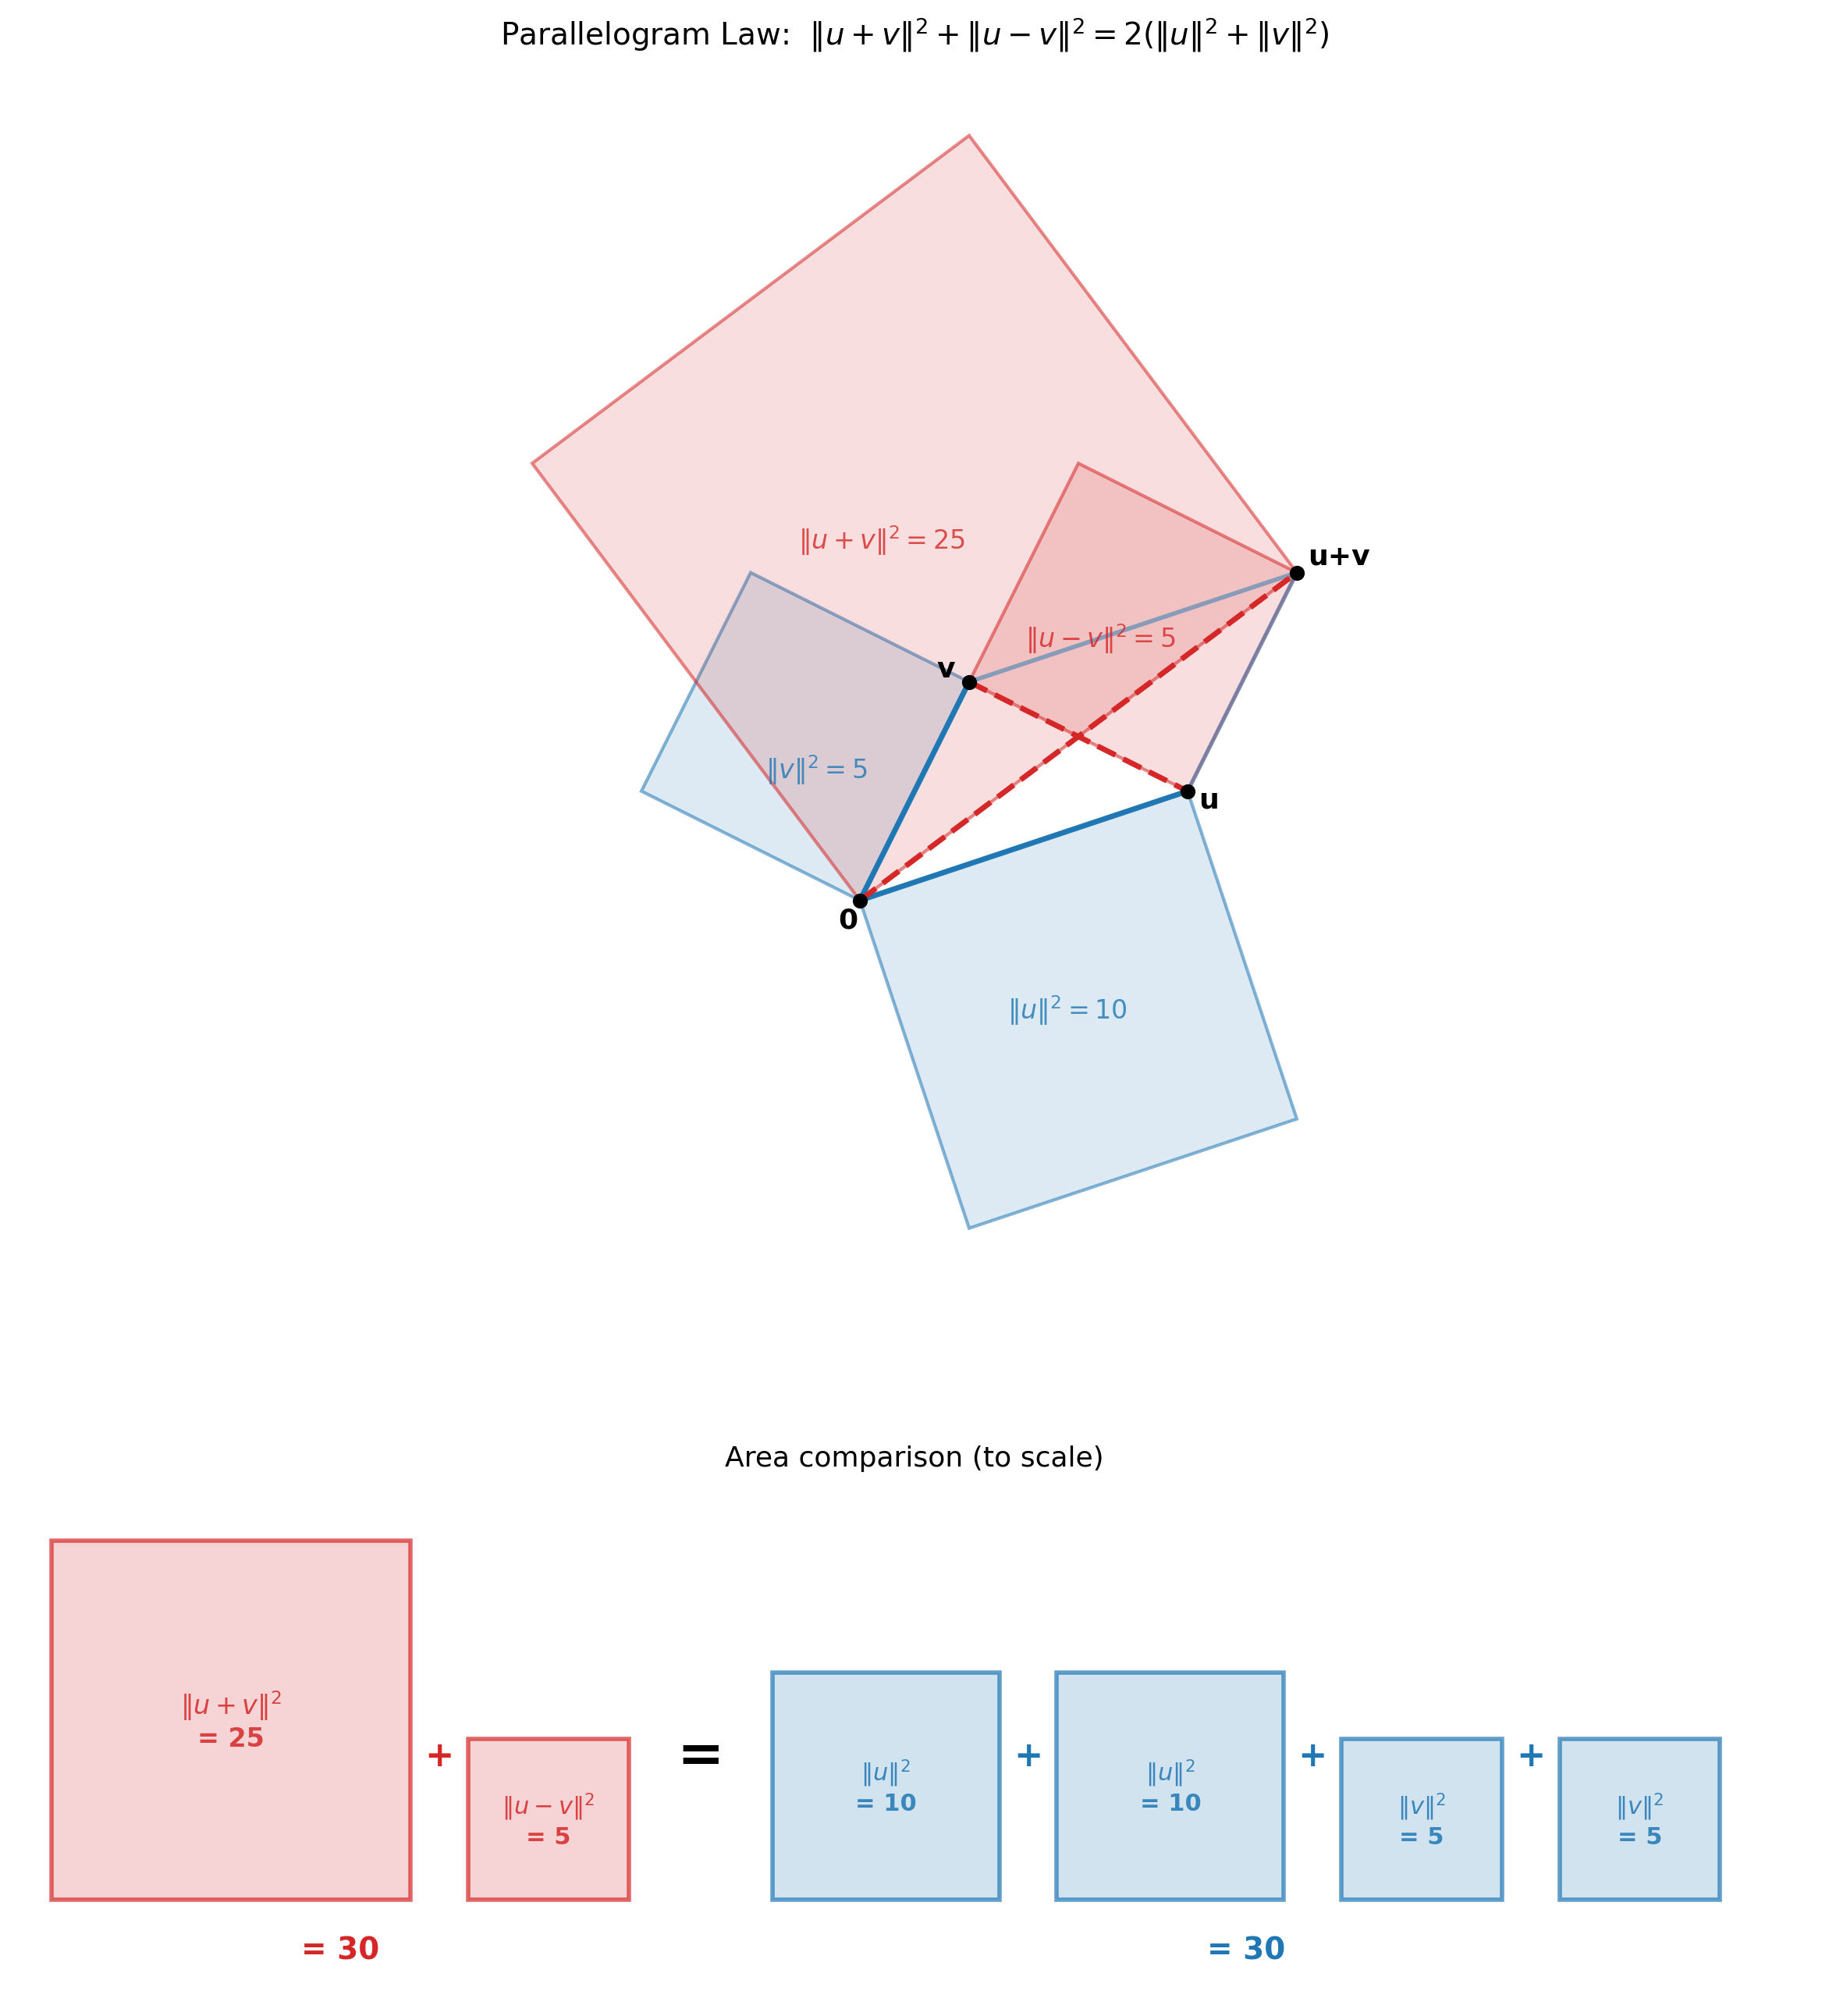
\includegraphics[width=0.85\textwidth]{parallelogram_law.png}
\caption{The parallelogram law illustrated. The areas of the squares built on the diagonals (red) sum to the same total as twice the areas of the squares built on the sides (blue). Any norm satisfying this identity must come from an inner product.}
\label{fig:parallelogram}
\end{figure}

\subsubsection*{Proof by direct expansion.}
The proof is short. In any inner product space, $\|w\|^2 = \langle w, w\rangle$, so we expand each diagonal:
\begin{align*}
\|u+v\|^2 &= \langle u+v,\; u+v\rangle \\
           &= \langle u,u\rangle + \langle u,v\rangle + \langle v,u\rangle + \langle v,v\rangle \\
           &= \|u\|^2 + 2\langle u,v\rangle + \|v\|^2,
\end{align*}
and similarly
\begin{align*}
\|u-v\|^2 &= \langle u-v,\; u-v\rangle \\
           &= \langle u,u\rangle - \langle u,v\rangle - \langle v,u\rangle + \langle v,v\rangle \\
           &= \|u\|^2 - 2\langle u,v\rangle + \|v\|^2.
\end{align*}
Adding the two expressions, the cross terms cancel:
\[
\|u+v\|^2 + \|u-v\|^2
= 2\|u\|^2 + 2\|v\|^2
= 2\bigl(\|u\|^2 + \|v\|^2\bigr). \qed
\]
Notice that the inner product $\langle u,v\rangle$ drops out entirely. The identity holds regardless of the angle between $u$ and $v$---it depends only on the existence of an inner product, not on its value.

\medskip

Why does this matter for statistics? In \(L^2\), the norm \(\|Z\| = (E[Z^2])^{1/2}\) comes from the inner product \(\langle Y, Z\rangle = E[YZ]\). Because this norm comes from an inner product, the parallelogram law holds, and with it the entire apparatus of projection geometry: the CEF can be characterized as a projection, the residual is orthogonal to every function of \(X\), and the variance decomposes cleanly. As we will see below, the parallelogram law is also the key ingredient in proving that such projections exist in the first place.

\medskip

By contrast, the conditional median minimizes absolute loss, but absolute loss is associated with \(L^1\), and \(L^1\) is not a Hilbert space. It is a normed space, but its norm does not come from an inner product. So there is no comparable projection geometry, no analogous orthogonality condition, and no variance decomposition of the same kind.

This is the deeper reason for the privileged status of the CEF: expectations live inside a mathematical framework that makes them especially easy to characterize, estimate, decompose, and interpret. The same logic helps justify the \emph{best linear predictor}: even when the true CEF is complicated, linear projections preserve much of this geometry while remaining tractable.

The CEF is the estimand that turns prediction into geometry.

\subsection*{Appendix: The Classical Projection Theorem}

\noindent\textit{This section sketches the proof for interested readers. The key takeaway is above: squared loss gives us an inner product, the parallelogram law, and therefore projection geometry.}

\medskip

One of the most important mathematical results in econometrics is the Classical Projection Theorem: the guarantee that, in a Hilbert space, every vector has a closest point in any closed subspace. This is the foundation for the CEF, the best linear predictor, and OLS. Its proof depends entirely on the parallelogram law---and therefore on the special structure of squared loss.

\medskip

\noindent\textbf{Theorem (Classical Projection).}
\textit{Let $H$ be a Hilbert space and $M$ a closed subspace of $H$. For any $x\in H$, there exists $m_0\in M$ such that}
\[
\|x - m_0\| \leq \|x - m\| \quad \text{for all } m\in M.
\]

\begin{proof}
If $x\in M$, take $m_0 = x$ and the result is immediate. So suppose $x\notin M$.

\medskip

\noindent\textbf{Step 1: Define the infimum.}
Let
\[
\delta = \inf_{m\in M} \|x - m\|.
\]
Since $x\notin M$ and $M$ is closed, $\delta > 0$. By the definition of infimum, there exists a sequence $\{m_i\}$ in $M$ such that
\[
\|x - m_i\| \to \delta \quad\text{as } i\to\infty.
\]

\medskip

\noindent\textbf{Step 2: The sequence is Cauchy (via the parallelogram law).}
Apply the parallelogram law to the vectors $u = x - m_i$ and $v = x - m_j$:
\[
\|u + v\|^2 + \|u - v\|^2 = 2\bigl(\|u\|^2 + \|v\|^2\bigr).
\]
Now observe that
\[
u + v = (x - m_i) + (x - m_j) = 2x - (m_i + m_j) = 2\!\left(x - \tfrac{m_i + m_j}{2}\right),
\]
and
\[
u - v = (x - m_i) - (x - m_j) = m_j - m_i.
\]
Substituting:
\[
\left\|2\!\left(x - \tfrac{m_i+m_j}{2}\right)\right\|^2 + \|m_j - m_i\|^2
= 2\bigl(\|x - m_i\|^2 + \|x - m_j\|^2\bigr).
\]
Pulling out the factor of $4$:
\[
4\left\|x - \tfrac{m_i+m_j}{2}\right\|^2 + \|m_i - m_j\|^2
= 2\|x - m_i\|^2 + 2\|x - m_j\|^2.
\]
Now the key observation: since $M$ is a subspace, $\frac{m_i + m_j}{2}\in M$, so $\|x - \frac{m_i+m_j}{2}\| \geq \delta$. Rearranging:
\[
\|m_i - m_j\|^2
= 2\|x - m_i\|^2 + 2\|x - m_j\|^2 - 4\left\|x - \tfrac{m_i+m_j}{2}\right\|^2
\leq 2\|x - m_i\|^2 + 2\|x - m_j\|^2 - 4\delta^2.
\]
As $i,j\to\infty$, both $\|x - m_i\|^2$ and $\|x - m_j\|^2$ converge to $\delta^2$, so the right-hand side converges to $2\delta^2 + 2\delta^2 - 4\delta^2 = 0$. Therefore $\|m_i - m_j\| \to 0$, and $\{m_i\}$ is Cauchy.

\medskip

\noindent\textbf{Step 3: Convergence.}
Since $H$ is complete (it is a Hilbert space) and $M$ is closed, the Cauchy sequence $\{m_i\}$ converges to some $m_0\in M$. By continuity of the norm,
\[
\|x - m_0\| = \lim_{i\to\infty} \|x - m_i\| = \delta.
\]
So $m_0$ achieves the infimum.
\end{proof}

\medskip

The proof reveals exactly where the parallelogram law does its work: in Step~2, it converts the statement ``$\frac{m_i+m_j}{2}$ is in $M$ and therefore at least $\delta$ away from $x$'' into a bound on $\|m_i - m_j\|$ that forces the minimizing sequence to be Cauchy. Without the parallelogram law---that is, without an inner product---this step fails, and a closest point need not exist. This is precisely why the CEF (a projection in $L^2$) is guaranteed to exist, while the analogous minimizer in $L^1$ is not.

(Uniqueness of $m_0$ can be shown separately by a similar argument: if $m_0$ and $m_0'$ both achieve the infimum, apply the parallelogram law to $u = x - m_0$ and $v = x - m_0'$ to conclude $\|m_0 - m_0'\| = 0$.)

\end{document}